\documentclass[a4paper,11pt,dvipdfmx]{ujarticle}
% パッケージ
\usepackage{graphicx}
\usepackage{url}
% レイアウト指定を記述したファイルの読み込み
\input{layout}

% タイトルと氏名を変更せよ.
\title{日本におけるデジタル化の状況}
\author{G584762025 廣島 修斗}

\begin{document}

\maketitle %

\section{ブロードバンドの設備状況}
% 節見出し: \section{日本におけるデジタル化の状況}
% を使う
OECDによるブロードバンド回線の普及に関する調査\cite{oecd}によると、図
\ref{1}に示すように、日本における 100人あたりのモバイルブロードバンドの
加入者数は190.5で、第1位になっている。2位はエストニア
で、3位米国と続く。
% 本文(1)
%  参考文献の参照: \cite{}
%  図番号の参照: \ref{}
% を使う
% 文献データベースのキーワードは oecd と imd
% になっている.
\begin{figure}[htbp]
    \centering
    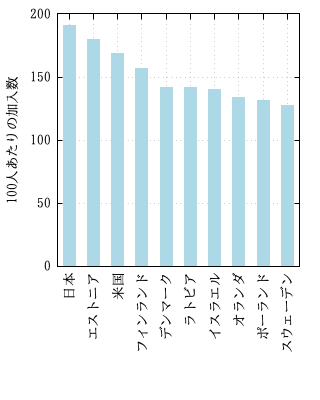
\includegraphics{fig21.png}
    \caption{光ファイバー回線の加入者数(100人あたり)}
    \label{1}
\end{figure}
% 図の挿入
% \includegraphics{}
% を
% \begin{figure}[htbp]
% \begin{figure}[htbp]
% で囲み
% \caption{}
% で図のタイトルを入れる.
% \label{}
% を使って図番号が参照できるようにする
% また,
% \centering
% で図が中央に来るようにする
\section{デジタル競争力ランキング}
% ーーー
% 節見出し(2)
国際経営開発研究所(IMD)の調査に\cite{imd}によると、
表\ref{2}にすように、日本のデジタル競争力のランキ
ングは調査対象の64カ国中、
総合で28位、知識分野で25位となっている。
% 本文(2)
\begin{table}[htbp]
    \centering
    \caption{デジタル競争力ランキング(64カ国中)}
    \label{2}
    \begin{tabular}{|c|c|c|}
        \hline
        国 & 総合 & 知識 \\
        \hline
        米国 & 1位 & 3位 \\
        \hline
        香港 & 2位 & 5位 \\
        \hline
        スウェーデン & 3位 & 2位 \\
        \hline
        デンマーク & 4位 & 8位 \\
        \hline
        シンガポール & 5位 & 4位 \\
        \hline
        \hline
        韓国 & 12位 & 15位 \\
        \hline
        中国 & 15位 & 6位 \\
        \hline
        \hline
        日本 & 28位 & 25位 \\
        \hline

    \end{tabular}
\end{table}

% 表の挿入
% \begin{tabular}
% \end{tabular}    
% による表の記述を 
% \begin{table}[htbp]
% \end{table}
% で囲み
% \caption{}
% で表のタイトルを入れる.
% \label{}
% を使って表番号が参照できるようにする
% また,
% \centering
% で表が中央に来るようにする

\section{考察}
\begin{itemize}
    \item 日本ではブローズバンドに加入しているが
    デジタル競争率は28位と低めになっていることから
    日本は技術が広まっているにもかかわらず技術開発に
    積極的ではないと考えられる。
    \item 逆にスウェーデンではブローズバンドが他国より
    あまり広まっていないにもかかわらずデジタル競争力は
    高くなっていることから技術開発を積極的に行っている
    と考えられる。
\end{itemize}
% ーーー
% 見出し(3)
% 考察
%
% \begin{itemize}
% \end{itemize}
% を使って箇条書きで記述する
% ここに参考文献が入る
%
\bibliographystyle{junsrt}
\bibliography{exercise.bib}

\end{document}